    
                %\title{LaTeX Portrait Poster Template}
%%%%%%%%%%%%%%%%%%%%%%%%%%%%%%%%%%%%%%%%%
% a0poster Portrait Poster
% LaTeX Template
% Version 1.0 (22/06/13)
%
% The a0poster class was created by:
% Gerlinde Kettl and Matthias Weiser (tex@kettl.de)
% 
% This template has been downloaded from:
% http://www.LaTeXTemplates.com
%
% License:
% CC BY-NC-SA 3.0 (http://creativecommons.org/licenses/by-nc-sa/3.0/)
%
%%%%%%%%%%%%%%%%%%%%%%%%%%%%%%%%%%%%%%%%%

%----------------------------------------------------------------------------------------
%   PACKAGES AND OTHER DOCUMENT CONFIGURATIONS
%----------------------------------------------------------------------------------------

\documentclass[a0,portrait]{a0poster}
%\setlength{\paperwidth}{33.1in}
%\setlength{\paperheight}{23.4in}

\usepackage[dutch]{babel}
\usepackage{enumitem}
\usepackage{apacite}
\renewcommand\bibliographytypesize{\tiny}
\usepackage{multicol} % This is so we can have multiple columns of text side-by-side
\columnsep=100pt % This is the amount of white space between the columns in the poster
\columnseprule=3pt % This is the thickness of the black line between the columns in the poster

\usepackage[svgnames]{xcolor} % Specify colors by their 'svgnames', for a full list of all colors available see here: http://www.latextemplates.com/svgnames-colors

\usepackage{times} % Use the times font
%\usepackage{palatino} % Uncomment to use the Palatino font

\usepackage{graphicx} % Required for including images
\usepackage{booktabs} % Top and bottom rules for table
\usepackage[font=small,labelfont=bf]{caption} % Required for specifying captions to tables and figures
\usepackage{amsfonts, amsmath, amsthm, amssymb} % For math fonts, symbols and environments
\usepackage{wrapfig} % Allows wrapping text around tables and figures


\begin{document}

%----------------------------------------------------------------------------------------
%   POSTER HEADER 
%----------------------------------------------------------------------------------------

% The header is divided into two boxes:
% The first is 75% wide and houses the title, subtitle, names, university/organization and contact information
% The second is 25% wide and houses a logo for your university/organization or a photo of you
% The widths of these boxes can be easily edited to accommodate your content as you see fit

\begin{minipage}[b]{0.4\linewidth}
\Huge \color{NavyBlue} \textbf{Bewustzijn heeft aandacht nodig}\\ \color{Black} % Title
\Large\textit{Gistperceptie onder dualtaskcondities}\\ % Subtitle
\end{minipage}
\begin{minipage}{0.4\linewidth}
\normalsize \textbf{Raoul Grouls\textsuperscript{1},
	\,Libby van den Besselaar\textsuperscript{2},
	\,Eva Bakels\textsuperscript{3},
	\,Kiki von Piekartz\textsuperscript{4}}\\ % Author(s)
\small Universiteit Utrecht,\,Kunstmatige Intelligentie,\,Nederland \\% University/organization
\small \texttt{(1) r.h.grouls@students.uu.nl}
\texttt{(2) l.l.m.vandenbesselaar@students.uu.n}\\
\texttt{(3) e.e.bakels@students.uu.nl}
\texttt{(4) k.g.piekartz@students.uu.nl}
\end{minipage}
\begin{minipage}[b]{0.2\linewidth}

\includegraphics[width=12cm]{uu-logo.png} 
\end{minipage}

\vspace{1cm} % A bit of extra whitespace between the header and poster content

%----------------------------------------------------------------------------------------

\begin{multicols}{3} % This is how many columns your poster will be broken into, a portrait poster is generally split into 2 columns

%----------------------------------------------------------------------------------------
%   ABSTRACT
%----------------------------------------------------------------------------------------

\color{Navy} % Navy color for the abstract

\begin{abstract}
bla die bla
\end{abstract}
%----------------------------------------------------------------------------------------
%   INTRODUCTION
%----------------------------------------------------------------------------------------

\color{Black} % SaddleBrown color for the introduction
\section*{Introductie}
Onderzoek heeft overtuigend aangetoond dat \textit{aandacht zonder bewustzijn} mogelijk is \cite{Jiang_Costello_Fang_Huang_He_2006, Sklar_Levy_Goldstein_Mandel_Maril_Hassin_2012, Cohen_Cavanagh_Chun_Nakayama_2012, Reddy_Reddy_Koch_2006, LiVanRullenKochPerona2002}. Onderwerp van discussie is echter de vraag of \textit{bewustzijn zonder aandacht} mogelijk is \cite{Cohen_Cavanagh_Chun_Nakayama_2012,Mack_Clarke_2012, Jennings_2015, Block_2011, Cohen_Dennett_2011, VanBoxtel_Tsuchiya_Koch_2010}. Een prominent onderdeel van deze discussie is onderzoek naar gistperceptie onder dualtask-condities gebruikt: \'{e}\'{e}n taak is ontworpen om de bestaande aandacht te monopoliseren, de andere taak onderzoekt het bewustzijn via gistperceptie (het waarnemen van de grote lijnen van een afbeelding die 30ms wordt getoond) \cite{Mack_Clarke_2012}.
\textbf{Aandacht} is daarbij gedefini\"eerd als  \textit{topdown, selectieve aandacht}. Door selectieve aandacht wordt informatie diepgaander verwerkt \cite{Cohen_Cavanagh_Chun_Nakayama_2012}. 
\textbf{Bewustzijn} verwijst naar de inhoud van bewustzijn en expliciet niet naar niveaus van bewustzijn zoals waken of slapen \cite{VanBoxtel_Tsuchiya_Koch_2010}.We hebben voor ons onderzoek de globale opzet van o.a. Mack \& Clarke (2012), Reddy et al. (2006) en Li et al. (2002) gebruikt: een dual-task opzet met een centrale aandachtstaak en perifere gistperceptie. Voor een aandachtstaak die schaalbaar is qua intensiteit hebben we de opzet met een \textit{multiple-object tracking task} overgenomen van Alvarez en Oliva (2008)\nocite{Alvarez_Oliva_2008}.\\

\color{Black} % DarkSlateGray color for the rest of the content

\section*{Hypothese}
De kritiek op bestaand onderzoek naar gistperceptie als onderbouwing voor \textit{bewustzijn zonder aandacht} is dat de aandachtstaak simpelweg niet intensief genoeg is \cite{Cohen_Alvarez_Nakayama_2011, Mack_Clarke_2012}. Deze onderzoeken laten zien dat proefpersonen de gist minder goed waarnemen, maar gebruiken als onafhankelijke variabele een \textit{aandachtsinstructie}. De proefpersonen mogen dan de aandachtstaak compleet los laten, om te zoeken naar de gistafbeelding. Dit is een belangrijke beperking, omdat hiermee onder andere oogbewegingen worden ge\"introduceerd die als contaminerende variabele kunnen optreden. Proefpersonen kunnen in de periferie namelijk minder detail waarnemen dan in het centrum van de focus\cite{moore2013clinically}. Dit kan voorkomen worden door de aandachtsinstructie constant te houden en als onafhankelijke variable de intensiteit van de aandachtstaak te vari\"eren. Ons onderzoek bekijkt de invloed van variatie in de aandachtstaak op de gistperceptie. Wij hypothetiseren het volgende:
\begin{quote}
\textit{Als aandacht een voorwaarde is voor bewustzijn, dan moet een aandachtstaak die toeneemt qua intensiteit leiden tot een verminderd bewustzijn van de gist. Wanneer aandacht geen voorwaarde is voor bewustzijn, zal het het bewustzijn van de gist gelijk blijven.}
\end{quote}
\begin{center}\vspace{1cm}
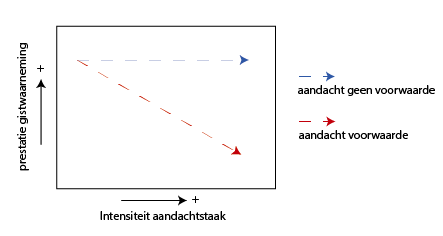
\includegraphics[width=1.0\linewidth]{illustratieHypothese.png}
\captionof{figure}{\color{Green} De visualisatie van onze hypothese: \'of aandacht een voorwaarde is voor bewustzijn wordt zichtbaar in de correlatie tussen gistperceptie en intensiteit van de aandachtstaak.}
\end{center}%\vspace{1cm}
%----------------------------------------------------------------------------------------
%   Methode
%----------------------------------------------------------------------------------------
\section*{Methode}

\textbf{Participanten} We hebben bij de selectie van proefpersonen (n=34) gestreefd naar een spreiding van leeftijd (mediaan=22, sd=15, range=17-60)en evenwichtige man/vrouw verhouding.(precies 1:1). We hebben bij de selectie rekening gehouden met de etniciteit van proefpersonen, omdat we verwachten dat dat mogelijk invloed kan hebben op het herkennen van de gezichten\cite{sporer2001recognizing}. \\
\textbf{Materiaal} Het experiment is opgezet met behulp van PsychoPy2 software\cite{peirce2007psychopy, Peirce2009generating} en geanalyseerd met R\cite{Rsoftware}. De complete code inclusief alle foto's zijn te vinden op GitHub \cite{Grouls2017}.\\
\textbf{Stimuli} Het een grijs scherm verschenen gedurende 6 seconden steeds 2 tot 4 ronde, blauwe objecten. Deze waren 5 pixels groot en volgden in zowel de x- als de y-richting een sinusgolf. De aandachtstaak van de proefpersonen was om te tellen hoe vaak de objecten de rode lijn kruisten. De bewustzijnstaak bestond uit het tegelijkertijd waarnemen van afbeeldingen met een mannen- of vrouwengezicht (zie Figuur 2). Het experiment werd voor elke conditie (2, 3 of 4 objecten) 20 keer herhaald, in een volledig \textit{mixed design} waarbij geen enkele conditie twee keer achter elkaar werd getoond. Na 6 seconden verscheen een rapportagescherm, waarbij proefpersonen voor de gistafbeelding konden kiezen uit 'man', 'vrouw' of 'geen afbeelding gezien' en voor de objecten konden rapporteren hoe vaak deze de rode lijn hadden gekruist.
\begin{center}\vspace{1cm}
	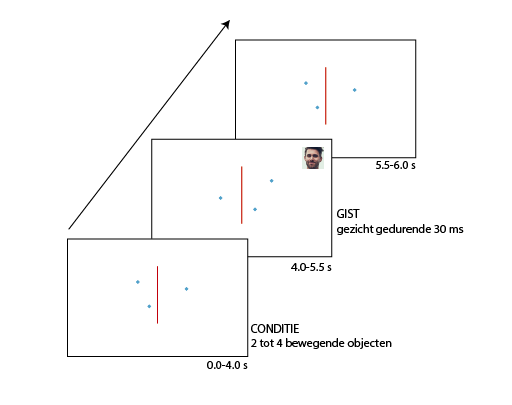
\includegraphics[width=0.8\linewidth]{Methode.png}
	\captionof{figure}{\color{Green} Schematische weergave van het experiment.}
\end{center}
\section*{Resultaten}
\textbf{Prestatie objecttelling} De eerste analyse die we hebben gedaan, was naar het percentage objecten dat de proefpersonen correct hadden geteld. Als de aandachtstaken inderdaad een textit{toenemende intesiviteit} hadden, dan moesten proefpersonen slechter scoren op conditie 4 dan op conditie 2. Hier is inderdaad het verwachte verloop zichtbaar (zie tabel 1), waarbij een conditie met meer objecten correleert met een lager percentage correct getelde objecten.
\begin{center}
	\captionof{table}{Prestatie objecttelling (in \%)}
\begin{tabular}{c c c c c}
	 &  mean  & SDM & min & max\\
	\hline
	conditie 2 & 95.16 & 0.65 & 81.47 & 100.00\\
	conditie 3 & 93.94 & 0.87 & 79.91 & 99.58\\
	conditie 4 & 89.37 & 1.10 & 71.05 & 96.58\\
	\hline\\
\end{tabular}
\end{center}
\textbf{Trainings- en vermoeidheidseffecten} Het viel ons echter op dat er ook andere patronen zichtbaar waren in de prestatie op de aandachtstaak. Wanneer we de ruwe data plotten voor prestatie op objecttelling, afgezet tegen het verloop in de tijd en differenti\"eren per conditie (fig. 3), valen twee dingen op:
\begin{enumerate}
	\item Alle lineaire regressies stijgen de eerste periode
	\item Na ongeveer 5 rondes (dus 15 experimenten) begint dit effect af te nemen en vermindert de score zelfs.
\end{enumerate}
 \begin{center}\vspace{1cm}
	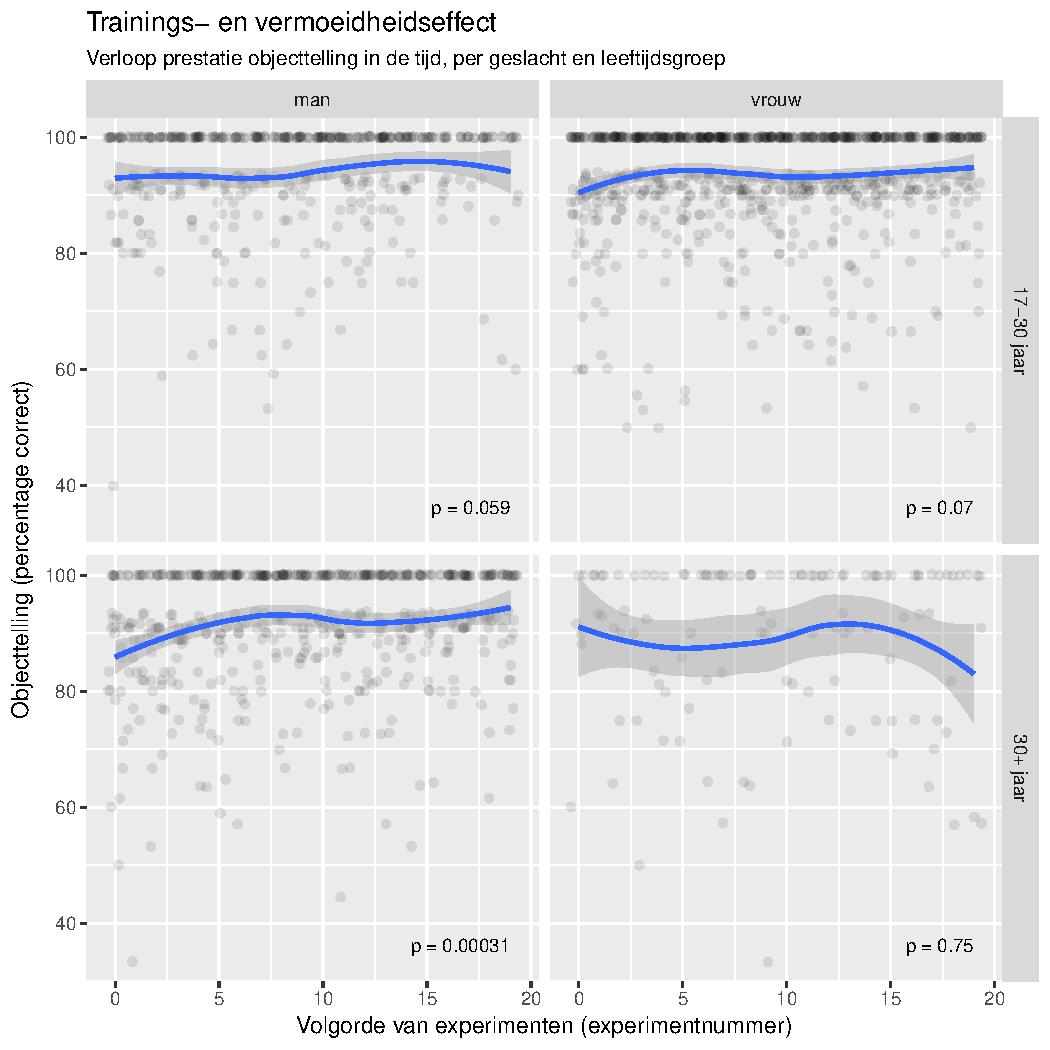
\includegraphics[width=0.8\linewidth]{training-grid.pdf}
	\captionof{figure}{\color{Green} De prestatie voor het correct tellen van de objecten uitgezet tegen het verloop in de tijd, uitgesplitst naar conditie.}
\end{center}\vspace{1cm}
We zien hier waarschijnlijk niet alleen een trainingseffect, maar ook een vermoeidheidseffect.Hoewel dit invloed heeft op het model, was deze invloed niet significant. We bespreken dit verder in de discussie.\\
\textbf{Prestatie gistwaarneming} Wanneer we de prestatie op de gistwaarneming uitzetten tegen de conditie in een boxplot (zie fig. 4), zien we duidelijk dat voor de conditie met 4 objecten het percentage correcte gistwaarneming daalt. In tabel 2 is duidelijk af te lezen dat de verschillen tussen conditie 2 en 4 significant zijn. 
\begin{center}
\captionof{table}{Prestatie gistwaarneming (in \%)}
\begin{tabular}{c c c c c}
	 &  mean  & SDM & min & max\\
	\hline
	conditie 2 & 91.08 & 1.17 & 70 & 100\\
	conditie 3 & 91.32 & 1.51 & 70 & 100\\
	conditie 4 & 85.98 & 1.71 & 60 & 100\\
	\hline\\
\end{tabular}
\end{center}
Wanneer we op deze resultaten een lineaire regressie toepassen volgens $f(x)=a x+b$, dan zou volgens onze hypothese een horizontale lijn (waarbij $a=0$) impliceren dat \textit{aandacht niet een voorwaarde} voor bewustzijn is. Een dalende horizontale lijn (waarbij $a<0$) zou impliceren dat \textit{aandacht wel een voorwaarde} voor bewustzijn is. Zoals duidelijk te zien is in figuur 5, is de lineaire regressie dalend (p = 0.017).
\begin{center}\vspace{1cm}
	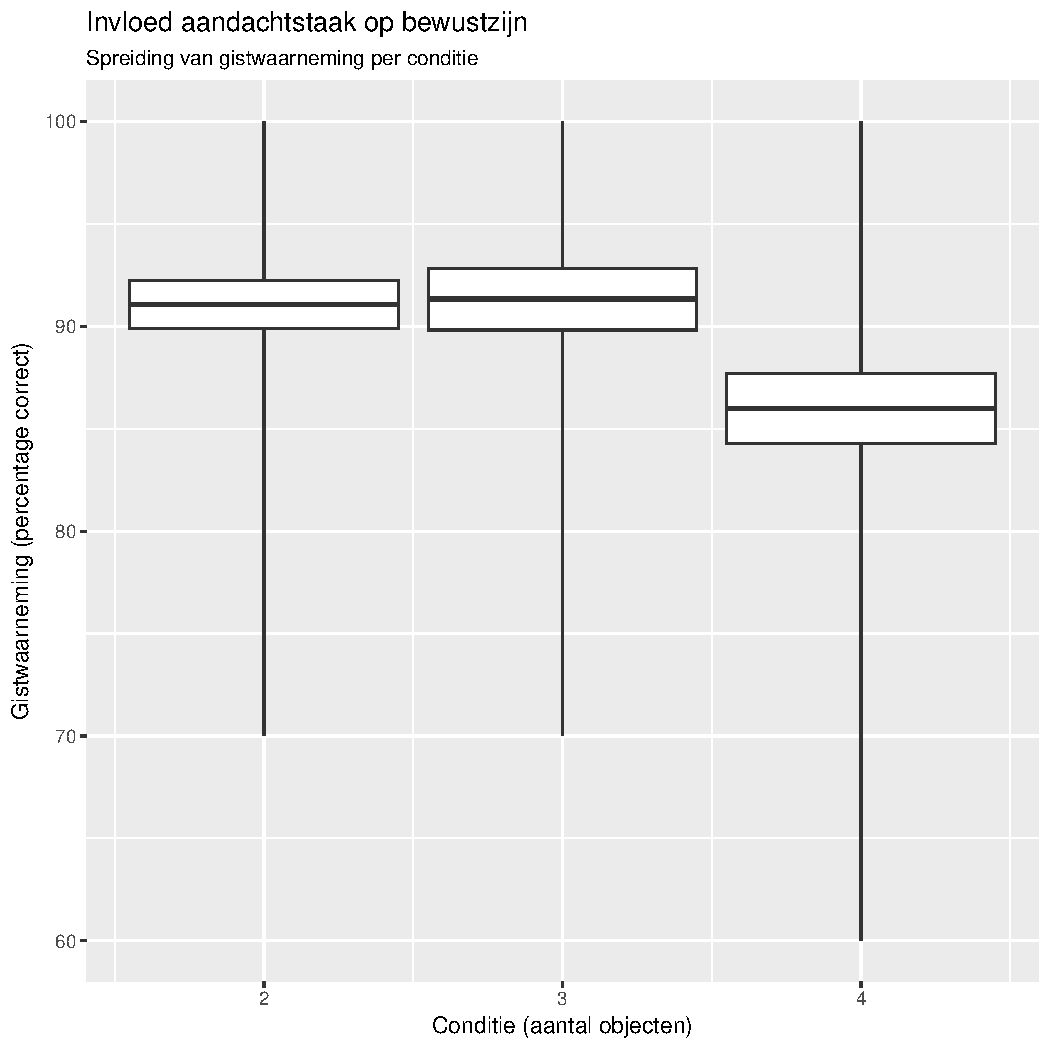
\includegraphics[width=0.8\linewidth]{boxplotGist-conditie.pdf}
	\captionof{figure}{\color{Green} Gistwaarneming per conditie. De errorbars geven de standaarddeviatie van het gemiddelde weer. De verticale lijn is de totale spreiding.}
\vspace{1cm}
	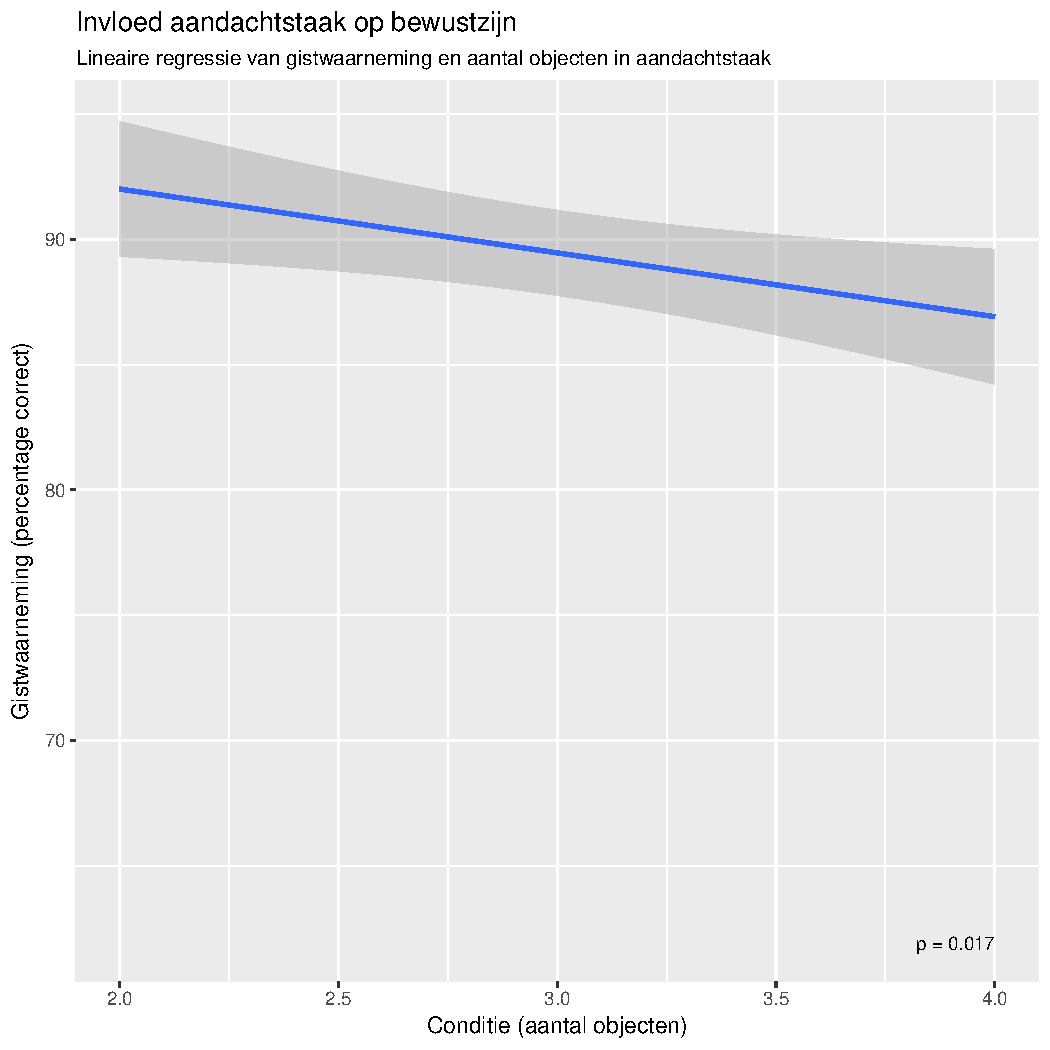
\includegraphics[width=0.8\linewidth]{lineaireRegressie.pdf}
	\captionof{figure}{\color{Green} De lineaire regressie volgens $f(x)=a x+b$}
\end{center}
\subsection*{Discussie}
Onze resultaten laten duidelijk zien dat de het bewustzijn afneemt wanneer de aandacht verder wordt gemonopoliseerd. Ondanks dat wij dit zelf niet hadden verwacht, was het resultaat 
 Er waren echter grote verschillen wat betreft dit vermoeidheidseffect tussen bijvoorbeeld mannen en vrouwen, of tussen de oudere leeftijdsgroep (30+) en de jongere leeftijdsgroep (17-30). Deze verschillen hebben invloed op de betrouwbaarheid van een lineair model $f(x)=a x+b$, omdat de monopoliseren van de aandacht na de 10e ronde tussen proefpersonen onderling sterk uiteen begon te lopen.
 \begin{center}
 \captionof{table}{invloed variatie in vermoeidheid op modelvorming}
\begin{tabular}{c c c}
	\hline
	p-waarde & $a$ & aantal rondes\\
	\hline
	0.007 & -0.035 & 9\\
	0.014 & -0.032 & 10\\
	0.043 & -0.024 & 15\\
	0.017 & -0.025 & 20\\
	\hline
\end{tabular}
 \end{center}

The total energy use for geothermal is about 1,778.65 TJ/yr.





%----------------------------------------------------------------------------------------
%   CONCLUSIONS
%----------------------------------------------------------------------------------------

\color{SaddleBrown} % SaddleBrown color for the conclusions to make them stand out

\section*{Conclusies}
Despite being a petroleum- and gas-rich country, 
\color{Black} % Set the color back to DarkSlateGray for the rest of the content

%----------------------------------------------------------------------------------------
%   FORTHCOMING RESEARCH
%----------------------------------------------------------------------------------------


 %----------------------------------------------------------------------------------------
%   REFERENCES
%----------------------------------------------------------------------------------------


%----------------------------------------------------------------------------------------
\bibliographystyle{apacite}
\bibliography{biblio}
\end{multicols}
\end{document}
              
            